% ------------------------------------------------------------------------ %
% !TEX encoding = UTF-8 Unicode
% !TEX TS-program = pdflatex
% !TEX root = ../Tesi.tex
% !TEX spellcheck = it-IT
% ------------------------------------------------------------------------ %
%
% ------------------------------------------------------------------------ %
% 	STATO DELL'ARTE
% ------------------------------------------------------------------------ %
%
\chapter{Stato dell'Arte Sanità Digitale} %Sanità Digitale in Italia
%
\label{cap:sanitàdigitale}
%
\section{Introduzione}
%
Con \emph{\enquote*{sanità digitale}} si intendono gli interventi condivisi da tutte le Amministrazioni operanti a livello centrale, regionale e locale per quanto riguarda: 
\begin{enumerate}
	\item la digitalizzazione del ciclo prescrittivo;
	\item la realizzazione di una soluzione federata di Fascicolo Sanitario Elettronico del cittadino;
	\item l’aumento del tasso di innovazione digitale nelle aziende sanitarie;
\end{enumerate}
In particolare, il \emph{Fascicolo Sanitario Elettronico} (FSE) è l’insieme dei dati e documenti digitali di tipo sanitario e socio-sanitario generati da eventi clinici presenti e trascorsi, riguardanti l’assistito. Ha un orizzonte temporale che copre l’intera vita del paziente ed è alimentato in maniera continuativa dai soggetti che lo prendono in cura nell’ambito del SSN\footnote{Sistema Sanitario Nazionale} e dei servizi socio-sanitari regionali ed è costituito, previo consenso dell’assistito, dalle Regioni e Province Autonome per le finalità di prevenzione, diagnosi, cura e riabilitazione perseguite dai soggetti del SSN e dei servizi sociosanitari regionali che prendono in cura l’assistito. È un investimento regionale, con una piattaforma FSE sovra-regionale. 
La normativa che regola la struttura del fascicolo è contenuta nel Decreto Legislativo 18/2012\cite{normaFSE} convertita, con modificazioni, dalla legge 17 dicembre 2012 del Decreto Legislativo 69/2013\autocite{decretofare}.\\
La \emph{Tessera sanitaria (TS)} invece, istituita ai sensi dell’articolo 50, comma 1, del decreto legge 269/2003, abilita all'accesso delle prestazioni sanitarie erogate dal SSN su tutto il territorio nazionale ed è Tessera di assicurazione malattia ai fini del riconoscimento dell'assistenza sanitaria nei Paesi UE, oltre a fungere da codice fiscale.\\
Infine, per quanto riguarda le \emph{Ricette digitali}, l’art. 50 della Legge 326/2003 (modificato dalla Legge finanziaria 2007) ha introdotto l’obbligo di trasmissione telematica dei dati delle ricette ai fini del controllo della spesa, ed il DL 78/2010 (art 11, comma 16)  ha dato valore legale alla trasmissione telematica dei dati delle ricette (scompare “ricetta rossa” cartacea). \\
Tutto il lavoro riguardante la sanità digitale in Italia è stato portato avanti dal gruppo di lavoro coordinato dall'AgID\footnote{Agenzia per l'Italia Digitale}, il quale ha rilasciato le Specifiche tecniche per l’interoperabilità tra i sistemi regionali del Fascicolo Sanitario Elettronico, comprendente il framework e dataset dei servizi base. Questo lavoro è stato il risultato dei test effettuati dalla Regione Emilia-Romagna, Lombardia e Veneto che, su proposta AgID, si sono offerte, con il supporto del CNR, di validare le specifiche di dettaglio per l’interoperabilità dei sistemi regionali di FSE ed in particolare i servizi di ricerca, recupero e indicizzazione dei documenti che compongono il Fascicolo. \\
Durante questa fase di progettazione inoltre, si è pronunciato anche il Garante della privacy \cite{garante} a tutela della protezione dei dati personali dei pazienti, per quanto riguarda il fascicolo sanitario elettronica e la refertazione online. Infatti, il garante ha deliberato che “il paziente deve poter scegliere, in piena libertà, se far costituire o meno un fascicolo sanitario elettronico, con tutte o solo alcune delle informazioni sanitarie che lo riguardano; deve poter manifestare un consenso autonomo e specifico, distinto da quello che si presta a fini di cura della salute; al paziente deve essere inoltre garantita la possibilità di "oscurare" la visibilità di alcuni eventi clinici. Per poter esprimere scelte consapevoli il paziente deve essere adeguatamente informato. Con un linguaggio comprensibile e dettagliato l'informativa deve quindi indicare chi (medici di base, del reparto ove è ricoverato, farmacisti) ha accesso ai suoi dati e che tipo di operazioni può compiere.
Il fascicolo sanitario elettronico potrà essere consultato dal paziente con modalità adeguate (ad es. tramite smart card) e dal personale sanitario strettamente autorizzato, solo per finalità sanitarie. Non potranno accedervi invece periti, compagnie di assicurazione, datori di lavoro.\\
%
\section{Fascicolo Sanitario Elettronico}
La realizzazione del Fascicolo Sanitario Elettronico in Italia ha visto, nel corso degli ultimi anni, uno sviluppo differenziato sul territorio nazionale a seconda dei contesti Regionali e Provinciali, nell'ambito dei quali alcune Amministrazioni hanno realizzato o avviato la realizzazione di infrastrutture di Fascicolo, mentre altre hanno sviluppato esperienze pilota significative. \\ 
In questo contesto le recenti modifiche al D.L. n\degree 179/2012 operate dal D.L. 69/2013\autocite{decretofare} e dalla successiva L. di conv. n\degree 98/2013, hanno dato un impulso decisivo alla realizzazione del Fascicolo Sanitario Elettronico sul territorio nazionale.\footnote{obbligatoria l'istituzione in tutte le Regioni italiane entro il 30 giugno 2015} \\
Le normative hanno inquadrato la fase implementativa nel seguente approccio:
\begin{enumerate}
	\item emanazione dello schema di DPCM attuativo per l'FSE;\cite{dpcmfse}
	\item emanazione, a cura dell’Agenzia per l’Italia Digitale e del Ministero della Salute, di Linee Guida dettagliate per il progetto del Fascicolo Sanitario Elettronico a partire dallo standard HL-7 \gls{EHR-SF};
	\item  presentazione del piano di progetto per la realizzazione del FSE da parte di ciascuna Regione e Provincia Autonoma.
\end{enumerate}
Nelle specifiche tecniche del fascicolo sanitario elettronico, scritte dall'AgID, si afferma che Il nucleo minimo del fascicolo, uguale per tutti i fascicoli istituiti da Regioni e Province autonome, è costituito dai seguenti dati e documenti:
\begin{enumerate}
	\item dati identificativi e amministrativi dell’assistito;
	\item referti;
	\item verbali pronto soccorso;
	\item lettere di dimissione;
	\item profilo sanitario sintetico;
	\item dossier farmaceutico;
	\item consenso o diniego alla donazione degli organi e tessuti;
\end{enumerate}
Il risultato più importante della fase di progettazione è stato la definizione di un modello funzionale del FSE\footnote{ ottenuto dalla localizzazione italiana dello standard ISO/HL7 EHR-S FM R2} al fine di evitare la proliferazione di sistemi funzionalmente incompatibili. Questo perchè le funzioni da realizzare devono essere conformi ad un modello funzionale di riferimento condiviso su scala nazionale e reimplementato a livello di singola regione. \\
Il modello così progettato, è diviso in due blocchi funzionali principali:
\begin{itemize}
	\item \emph{Servizi di interfaccia}: consentono l’interazione da parte degli attori e delle componenti esterne con il sistema di FSE regionale. Ci sono ad esempio i servizi di interfaccia interregionale;
	\item \emph{Macro funzioni}: raccolgono le funzioni del modello logicamente correlate. Tra queste funzioni troviamo ad esempio le funzioni di indicizzazione dei documenti, quelle di alimentazione, quelle per la sicurezza e la privacy etc.
\end{itemize}
La struttura generale infatti è la seguente:
%
\begin{center}
	%
	\begin{figure}[tbhp]
		%
		\centering
		%
		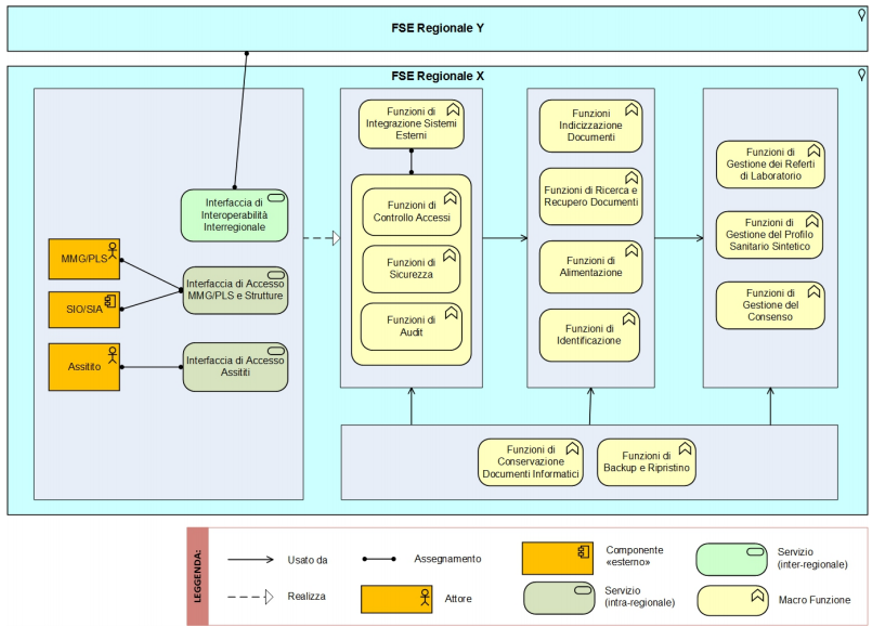
\includegraphics[width=.9\textwidth]{Sanitadigitale/fse}
		%
		\caption{Modello funzionale FSE}
		%
		\label{fig:modelloFSE}
		%
	\end{figure}
	%
\end{center}
%
Mentre le principali fonti di informazioni che il Fascicolo Sanitario Elettronico raccoglie sono le seguenti:
%
\begin{center}
	%
	\begin{figure}[tbhp]
		%
		\centering
		%
		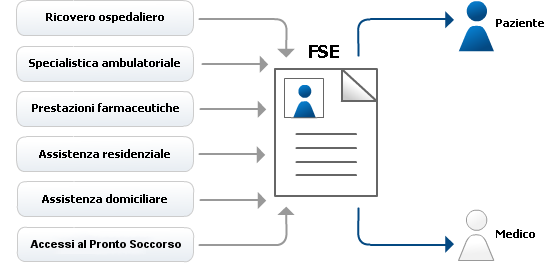
\includegraphics[width=.9\textwidth]{Sanitadigitale/fse2}
		%
		\caption{Schema dei dati raccolti dal FSE}
		%
		\label{fig:schema dati fse}
		%
	\end{figure}
	%
\end{center}
%
% In particolare nei servizi di interfaccia troviamo:
% \begin{itemize}
% 	\item \emph{Interfaccia di Interoperabilità Interregionale}: questa interfaccia rappresenta il punto di accesso ai servizi esposti dai sistemi regionali di FSE che consentono a questi ultimi di interoperare tra loro;
% 	\item \emph{Interfaccia di Accesso MMG/PLS e Strutture}: questa interfaccia consente alle strutture sanitarie e ai MMG/PLS di accedere ed utilizzare il sistema regionale di FSE;
% 	\item \emph{Interfaccia di Accesso Assistiti}: l’interfaccia offre la possibilità agli assistiti di accedere ed utilizzare il FSE;
% \end{itemize}
% Invece le macro funzioni sono state raggruppate nel seguente modo:
% \begin{enumerate}
% 	\item \emph{Funzioni di Integrazione Sistemi Esterni}: il sistema FSE deve predisporre una serie di funzioni che permettano l’utilizzo di servizi esposti da sistemi esterni, come ad esempio il servizio di anagrafe o il sistema di prenotazione delle prestazioni;
% 	\item \emph{Controllo Accessi}: tutti gli attori e le componenti esterne del sistema di FSE devono essere autenticate ed autorizzate da parte del sistema per poter accedere ed utilizzare i servizi messi a disposizione (funzioni di controllo accessi a livello regionale-nazionale);
% 	\item \emph{Sicurezza}: il sistema di FSE deve comprendere una serie di funzioni di supporto alla sicurezza, ad esempio per assicurare lo scambio sicuro dei dati e la tutela della privacy dell’assistito;
% 	\item \emph{Audit}: il sistema di FSE deve tracciare tutte le operazioni effettuate, mediante la memorizzazione e la gestione degli eventi di interesse;
% 	\item \emph{Funzioni Indicizzazione Documenti}: il sistema di FSE deve predisporre una serie di funzioni che consentano di indicizzare, mediante opportuni metadati, i documenti e dati prodotti dalle strutture sanitarie o socio-sanitarie (o condivisi dall’assistito);\footnote{I metadati hanno l’obiettivo di descrivere e di consentire il reperimento (mediante puntatori) dei documenti e dati prodotti sia all’interno che all’esterno del dominio regionale}
% 	\item \emph{Funzioni di Ricerca e Recupero Documenti}: i documenti e dati disponibili nel FSE devono essere facilmente reperibili da parte degli utenti autorizzati tramite opportune funzioni integrate nel sistema;
% 	\item \emph{Funzioni di Alimentazione}: il sistema di FSE deve mettere a disposizione funzioni che consentano agli attori autorizzati l’inserimento di dati e documenti nel sistema di FSE;
% 	\item \emph{Funzioni di Identificazione}: il sistema di FSE deve fornire una serie di funzioni per la gestione dell’identificazione dell’assistito, del professionista sanitario, del MMG/PLS e delle strutture sanitarie;
% 	\item \emph{Gestione Referti di Laboratorio}: il sistema di FSE deve fornire una serie di funzioni per la gestione dei referti di laboratorio;
% 	\item \emph{Gestione Profilo Sanitario Sintetico}: il sistema di FSE deve fornire funzioni atte alla gestione del Profilo Sanitario Sintetico;
% 	\item \emph{Gestione Consenso}: il sistema di FSE deve offrire una serie di funzionalità per la gestione di due tipologie di consenso da parte dell’assistito: consenso all’alimentazione e consenso alla consultazione dei dati e documenti del FSE;
% 	\item \emph{Backup e Ripristino}: il sistema di FSE deve fornire funzionalità trasversali a tutte le altre funzioni offerte, al fine di consentire la gestione di copie di sicurezza dei dati e documenti presenti nel FSE, la continuità ed il ripristino dei servizi erogati dai sistemi regionali.
% 	\item \emph{Conservazione Documenti Informatici}: il sistema di FSE deve rispettare le regole per la conservazione dei documenti e dati informatici (con riferimento ai documenti e dati di propria competenza, quali metadati componenti l’indice, informazioni condivise dall’assistito nel taccuino, dati relativi al consenso, ecc.), per il periodo di tempo previsto dalla normativa vigente;
% \end{enumerate}
La realizzazione di sistemi di FSE così strutturati costituisce, a livello regionale, un salto di notevole importanza per il miglioramento dell’efficacia ed efficienza delle cure percepite dai cittadini all’interno di un sistema sanitario regionale rispetto al modello precedente basato su registri e cartelle cartacee e blocchi di prescrizione stampati dalla zecca di Stato e consegnati personalmente ad ogni medico del distretto sanitario di appartenenza. \\
Una delle fonti di informazioni maggiori del Fascicolo Sanitario Elettronico, che è anche oggetto di studio in questo lavoro di tesi, risulta essere composta dall'insieme delle prescrizioni che i medici generano per i propri pazienti e che vengono erogate dalle farmacie presenti sul territorio nazionale. Il governo ha inoltre lasciato libertà di implementazione e gestione delle strutture alle singole regioni portando così alla creazione di sistemi eterogenei che fanno capo ad alcuni punti di riferimento gestiti dal Governo tramite le infrastrutture della Sogei. Il sistema complessivo si presenta come un sistema di tipo centralizzato caratterizzato dalle tipiche problematiche dei central points of failure. Inoltre, per quanto riguarda il sistema delle prescrizioni, esso gestisce solo le ricette mediche \emph{rosse} mentre le ricette mediche bianche non sono oggette ancora di prescrizione elettronica in tutte le regioni. Le funzionalità da cui si è partito per sviluppare questo lavoro di Tesi sono quelle riguardanti la prescrizione e l'erogazione delle ricette mediche \emph{bianche} che differiscono dalle ricette mediche rosse per una serie di caratteristiche che saranno illustrate nel proseguio del capitolo.
%
\section{Ricetta Elettronica}
%
Parallelamente al processo di istituzione del Fascicolo Sanitario Elettronico, anche il sistema di prescrizione farmaceutica è, al momento, oggetto di grandi modifiche in quanto sta diventando digitale. \\
Infatti, attraverso il \emph{Sistema Tessera Sanitaria} (TS), è stata realizzata la diffusione della ricetta elettronica, con la \gls{dematerializzazione} delle ricette mediche, introdotta con il D.L. n\degree 78/2010, il decreto ministeriale del 2/11/2011 ed il D.L. n\degree 179/2012. \cite{agendadigitale} Questo sistema è il sistema informativo centralizzato, realizzato in attuazione dell'art 50 del D.L. 269/2003, dal Ministero dell'economia e delle finanze - Ragioneria Generale dello Stato e gestito per la parte informatica da Sogei\footnote{Società di Information Technology interamente controllata dal Ministero dell'Economia e delle Finanze}.
La ricetta elettronica prevede la completa eliminazione del supporto cartaceo della ricetta nell’intero iter che va dalla fase di prescrizione del medico, alla erogazione della prestazione, al successivo controllo e rendicontazione. \\
Le finalità del progetto sono:
\begin{itemize}
	\item potenziamento dei controlli e prevenzione errori nelle prescrizioni;
	\item maggiore interscambio di informazioni favorito dal formato digitale;
	\item semplificazioni accesso prestazioni sanitarie a carico del SSN;
\end{itemize}
La prescrizione elettronica quindi, si presenta come il primo importante tassello nella costruzione del FSE in quanto rappresenta una delle porzioni più importanti dei dati clinici del paziente.\\
Esistono due tipi principali di ricette:
\begin{itemize}
	\item \emph{\gls{ricetta rossa}}: può essere compilata solamente dai medici dipendenti di strutture pubbliche o convenzionati con il servizio sanitario nazionale e viene utilizzata per la prescrizione di una terapia farmacologica, la prescrizione di un esame diagnostico o una visita specialistica a carico del servizio sanitario. L’uso di una ricetta rossa non permette l’erogazione a carico del servizio sanitario di farmaci o prodotti parafarmaceutici non compresi tra le formulazioni del prontuario farmaceutico regionale, né di esami, visite o terapie non comprese nei Lea o nelle disposizioni della propria regione. Un esempio è illustrato nella seguente figura:
	      %
	      \newline
	      %
	      \begin{figure}[h!]
	      	%
	      	\centering
	      	%
	      	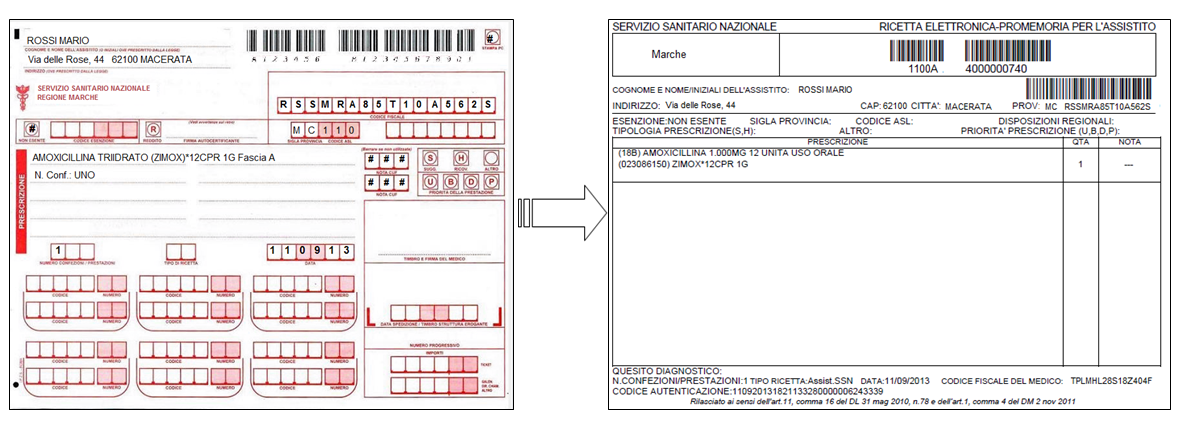
\includegraphics[width=1.0\textwidth]{Sanitadigitale/ricetta}
	      	%
	      	\caption{Ricetta rossa dematerializzata}
	      	%
	      	\label{fig:Ricetta rossa dematerializzata}
	      	%
	      \end{figure}
	      %
	      \newline
	      %
	\item \emph{\gls{ricetta bianca}}: ricetta che il medico compila su carta bianca, sulla quale siano però riportati: il nome e cognome del medico; la data; il luogo; la firma autografa del medico. In questo caso, il nome dell’assistito non è strettamente necessario. Su ricetta bianca possono essere prescritte tutte le prestazioni di specialistica ambulatoriale, di diagnostica strumentale e di laboratorio, di norma correlate alla propria branca di specializzazione e i farmaci, prestazioni che saranno sempre a carico del cittadino assistito. Per la prescrizione a carico del servizio sanitario è infatti necessaria la ricetta del ricettario regionale ed è valida in tutte le farmacie italiane. Una delle attuali criticità del sistema è che il procedimento della dematerializzazione delle ricette non si applica per le ricette bianche che vengono ancora compilate su normale carta:
	      \begin{center}
	      	%
	      	\begin{figure}[tbhp]
	      		%
	      		\centering
	      		%	      		      	
	      		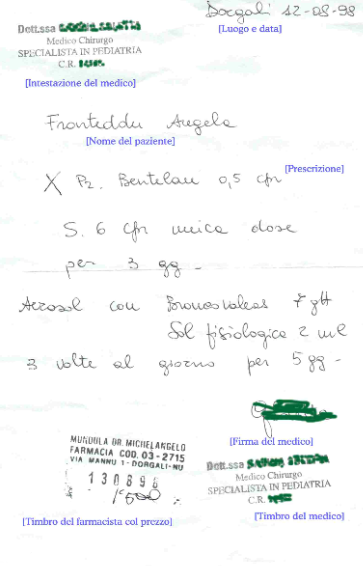
\includegraphics[width=0.5\textwidth]{Sanitadigitale/ricettaBianca}
	      		%
	      		\caption{Ricetta bianca}
	      		%
	      		\label{fig:Ricetta bianca}
	      		%
	      	\end{figure}
	      	%
	      \end{center}
\end{itemize}
%
\section{Architettura del Sistema}
%
L'attività di accoglienza dei dati delle ricette prescritte, prevede l'utilizzo di due sistemi centrali:
\begin{enumerate}
	\item \emph{Sistema di accoglienza} (SAC): è il Sistema di Accoglienza Centrale gestito da Sogei per il Ministero dell'Economia e delle Finanze (MEF). Il SAC gestisce la circolarità nazionale delle ricette dematerializzate, ovvero la possibilità per gli assistiti di utilizzare una prescrizione in qualunque Regione, garantendo anche che la stessa prestazione non sia erogata più volte in regioni diverse;
	\item \emph{Sistema di accoglienza regionale} (SAR): è il Sistema di Accoglienza Regionale gestito da CUP 2000 che colloquia con il Sistema di Accoglienza Centrale del Ministero (SAC) per l’invio e il recupero delle ricette dematerializzate, ed aggiorna lo stato della ricetta (prenotata, sospesa,bloccata ed erogata) E' in grado di: \begin{itemize}
	\item raccogliere tutte le prescrizioni dematerializzate inviate dai medici prescrittori della Regione;
	\item rendere disponibili le prescrizioni dematerializzate ai sistemi che, se abilitati, possono accedere alla ricetta stessa (CUP, accettazioni, farmacie, etc.);
	\item fornire servizi di ritorno informativo verso le Aziende sanitarie e le farmacie;
	\item sviluppare le regole e i controlli regionali necessari a garantire l’emissione di prescrizioni corrette;
	\end{itemize}
\end{enumerate}
Questi due sistemi coesistono contemporaneamente, in quanto nel caso in cui le regioni non avessero sviluppato un proprio sistema di accoglienza, il SAC si configura come sistema di riferimento per i medici prescrittori, le farmacie e le strutture di erogazione di prestazioni di specialistica ambulatoriale, generando per questi le credenziali di accesso al sistema\footnote{abilitazione al SAC. Credenziali inviate tramite busta chiusa alle ASL territoriali}. Invece nel caso in cui la regione abbia a disposizione un SAR proprio, esso si andrà ad interfacciare con il SAC, che fungerà da secondo centro di accoglienza con le stesse funzionalità del SAR, solamente estese a livello nazionale.
%
\subsection{Caso di studio: Regione Marche}
%
Nella Regione Marche, la delibera 677\cite{drmarche} della Giunta Regionale 04/06/2014 per l'approvazione dello "schema di protocollo di intesa con i medici di medicina generale per la riqualificazione della medicina del territorio e la messa a regime della rete regionale per la ricetta dematerializzata e per l'implementazione dei flussi di dati" che ha dato il via al progetto di dematerializzazione delle ricette SSN il quale prevede la sostituzione della ricetta rossa cartacea con la ricetta elettronica dematerializzata. La procedura per l'emissione di una ricetta è la seguente:
\begin{itemize}
	\item il medico prescrittore:
	      \begin{enumerate}
	      	\item si collega al Sistema Centrale Tessera Sanitaria (anche attraverso un eventuale SAR)\footnote{essendo nelle Marche presente anche il SAR, la comunicazione avviene verso il SAR e poi verso il SAC e successivamente viene effettuato un controllo incrociato delle informazioni inserite nei due sistemi};
	      	\item genera i dati della ricetta elettronica. Il contenuto della ricetta viene salvato nel Sistema Tessera Sanitaria a livello centrale (tenuto sempre conto che il contenuto sarà anche salvato nel SAR, se presente). La ricetta sarà identificata tramite un codice univoco nazionale denominato \emph{Numero di Ricetta Elettronica} (NRE) e conterrà i seguenti elementi: NRE, dati anagrafici dell'assistito titolare della prescrizione, eventuali esenzioni e la prestazione da erogare;
	      	\item se i dati risultano corretti, il medico rilascia al paziente un \emph{promemoria} cartaceo contenente i dati della ricetta dematerializzata;
	      \end{enumerate} 
	\item la struttura erogatrice:
	      \begin{enumerate}
	      	\item presso la struttura erogatrice, l'assistito presenterà il promemoria;
	      	\item la struttura si collegherà al sistema centrale (SAR o SAC) e procederà alla ricerca della ricetta attraverso l'NRE riportato su di essa, unitamente al codice fiscale dell'assistito riportato sulla sua tessera sanitaria;
	      	\item nel caso in cui la ricetta risulti erogabile, la struttura procede all'erogazione della prestazione comunicando al tempo stesso le informazioni sulla prestazione erogata (al SAR e/o al SAC);
	      	\item completata l'erogazione la struttura ritira il promemoria al paziente;
	      \end{enumerate}
\end{itemize}
Questa sequenza viene mostrata nella figura seguente:
%
\begin{figure}[H]
	%
	\centering
	%
	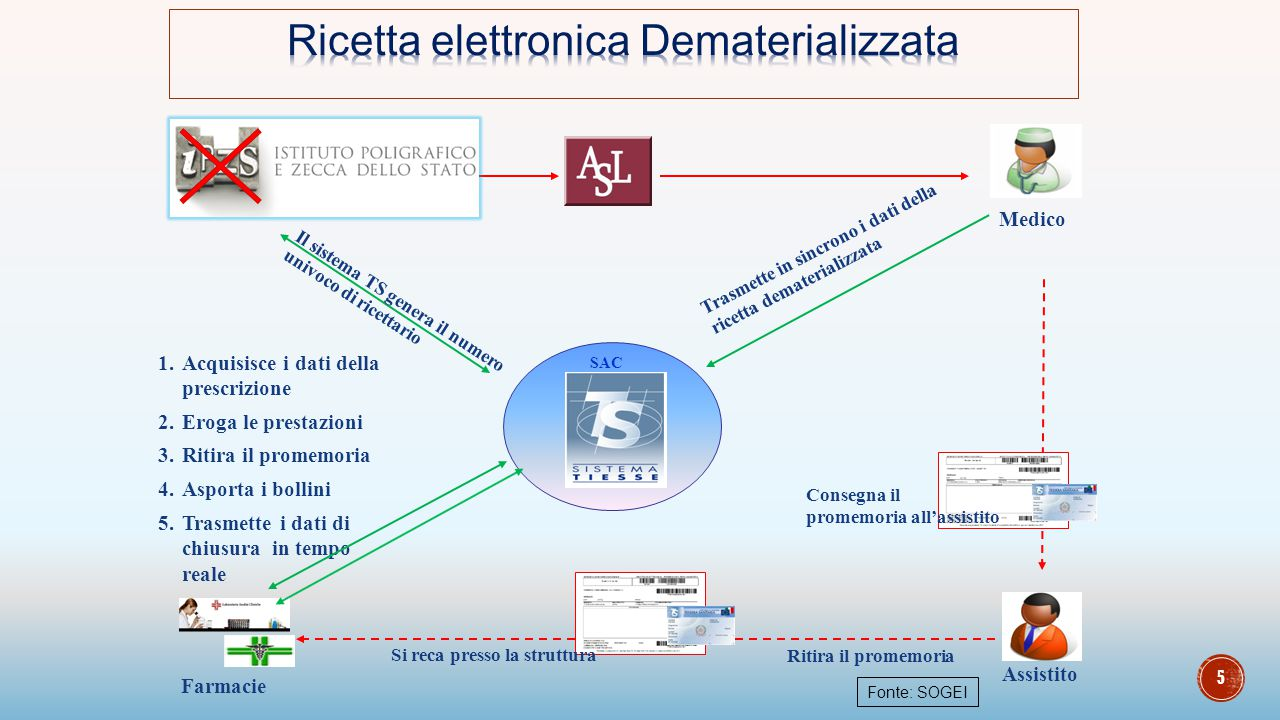
\includegraphics[width=.9\textwidth]{Sanitadigitale/erogazioneRicetta}
	%
	\caption{Diagramma dell'erogazione di una ricetta}
	%
	\label{fig:Erogazione di una ricetta dematerializzata}
	%
\end{figure}
%
Il complesso dei servizi offerti dal FSE nell'ambito della Regione Marche è garantito da un insieme di componenti applicative cooperanti tra loro supportate da un apparato infrastrutturale allocato presso il data center sanità e i nodi aziendali, il tutto integrato all’interno di un contesto regionale caratterizzato dall’esistenza di sistemi preesistenti, con cui il FSE si troverà ad interagire  per l’esposizione dei propri servizi rispetto al SAC centrale. Le componenti sono eterogenee e sono riassunte nella seguente figura:
%
\begin{figure}[H]
	%
	\centering
	%
	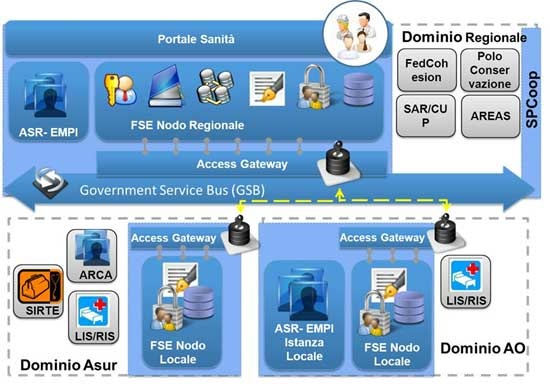
\includegraphics[width=.9\textwidth]{Sanitadigitale/sanitaMarche}
	%
	\caption{Schema architetturale sanità digitale Marche}
	%
	\label{fig:Schema architetturale sanità digitale Marche}
	%
	\vfill
\end{figure}
%
\section{Una soluzione decentralizzata}
%
\subsection{Criticità del sistema}
Questo sistema ha dimostrato alcune criticità a seguito delle sperimentazioni fatte e dell'attuale utilizzo:
\begin{itemize}
	\item la mancanza di collegamenti internet o di una piattaforma di gestione troppo lenta in alcune zone crea problemi di utilizzo e di sovraccario del sisstema;
	\item la presenza di due distinti sistemi di trasmissione dati e accoglienza delle ricette (SAC/SAR) ha aggiunto un ulteriore grado di complessità alle architetture dei sistemi a livello regionale ed inter-regionale in quanto alcune regioni hanno optato per l'utilizzo del SAC mentre altre del SAR (che si interfaccia con il SAC). Inoltre, normalmente un SAR risulta essere più lento di un SAC a livello di gestione del flusso dei dati;
	\item la prescrizione delle ricette bianche risulta essere esclusa dalla dematerializzazione. Quindi una ricetta bianca può essere oggetto di falsificazione o truffa, nel caso in cui il blocco di ricette con i dati del medico venga rubato;
\end{itemize}
Inoltre, possono verificarsi casi in cui i server di Sogei del SAC responsabili della prescrizione e spedizione della ricetta digitale risultino irragiungibili con conseguenze che vanno dal mancato invio della ricetta digitale al non poter verificare la veridicità del contenuto di un promemoria se non in modo "postumo" all'erogazione del contenuto della prescrizione cartacea.
%
\subsection{La decentralizzazione}
Una possibile soluzione di queste criticità può essere trovata nell'utilizzo di un approccio decentralizzato che risiede nell'utilizzo della blockchain (si eliminano i Single Point of Failure) per registrare gli eventi (che saranno organizzati in blocchi) e le transazioni di prescrizione ed erogazione.  L'utilizzo della blockchain ci garantisce:
\begin{itemize}
	\item \emph{Non ripudio}: la decisione riguardante la validità di un’informazione non viene presa unilateralmente ma attraverso un meccanismo di raccolta del consenso all’interno della rete, rendendo così particolarmente difficile metterne in discussione l’esito;
	\item \emph{Autenticità}: tutti gli eventi possono essere fatti risalire con certezza alle identità digitali che li hanno generati, attraverso l’utilizzo di meccanismi di crittografia asimmetrici;
	\item \emph{Integrità}: i dati che sono stati scritti all’interno della Blockchain non possono essere modificati, se non attraverso specifiche regole del protocollo che definiscono rigorosamente le modalità con cui si possono effettuare cambiamenti;
	\item \emph{Tracciabilità}: a tutti gli eventi registrati vengono assegnati un identificativo e una marca temporale che li rende facilmente tracciabili e verificabili.
	\item \emph{Programmabilità}: all’interno dei blocchi possono essere incluse istruzioni che facciano scatenare specifiche azioni al verificarsi certe condizioni.
\end{itemize}
